\section{设计}

\subsection{设计挑战}

尽管 \DAP{} 原则在概念上相对简单，但在 LLM 服务场景中将其真正落地并不容易。\sys{} 必须在\emph{信息不完备}的情况下进行优先级分配：在缺乏精确松弛度的前提下，通过\emph{离散多级队列}（例如交换机上的有限优先级队列）来引导流。具体而言，我们识别出以下两个挑战。

\parab{C-1：如何在不过度优先的前提下调度带显式截止时间的流。}
即便某些流携带显式截止时间（如 P2D 传输），在离散优先级层级下，何时从“延后”切换到“提升”仍然并不简单。过早提升会浪费稀缺的瓶颈带宽，而过晚提升则会导致截止违约。难点在于：在有限优先级类别下，如何找到“恰好按时完成”的平衡点。

\parab{C-2：如何在没有精确松弛度的情况下调度隐式截止时间流。}
缺乏精确松弛度会让调度器陷入容易出错的两难。一方面，若低估松弛度，就会带来意外的执行停顿：误将阶段 2 流延后会立即让 GPU 空转，并拉长请求延迟。另一方面，若高估松弛度，则会造成优先级反转，把稀缺带宽浪费在本可延后的工作上，使真正紧急的请求被饿死。

\begin{figure}[t!]
    \centering
    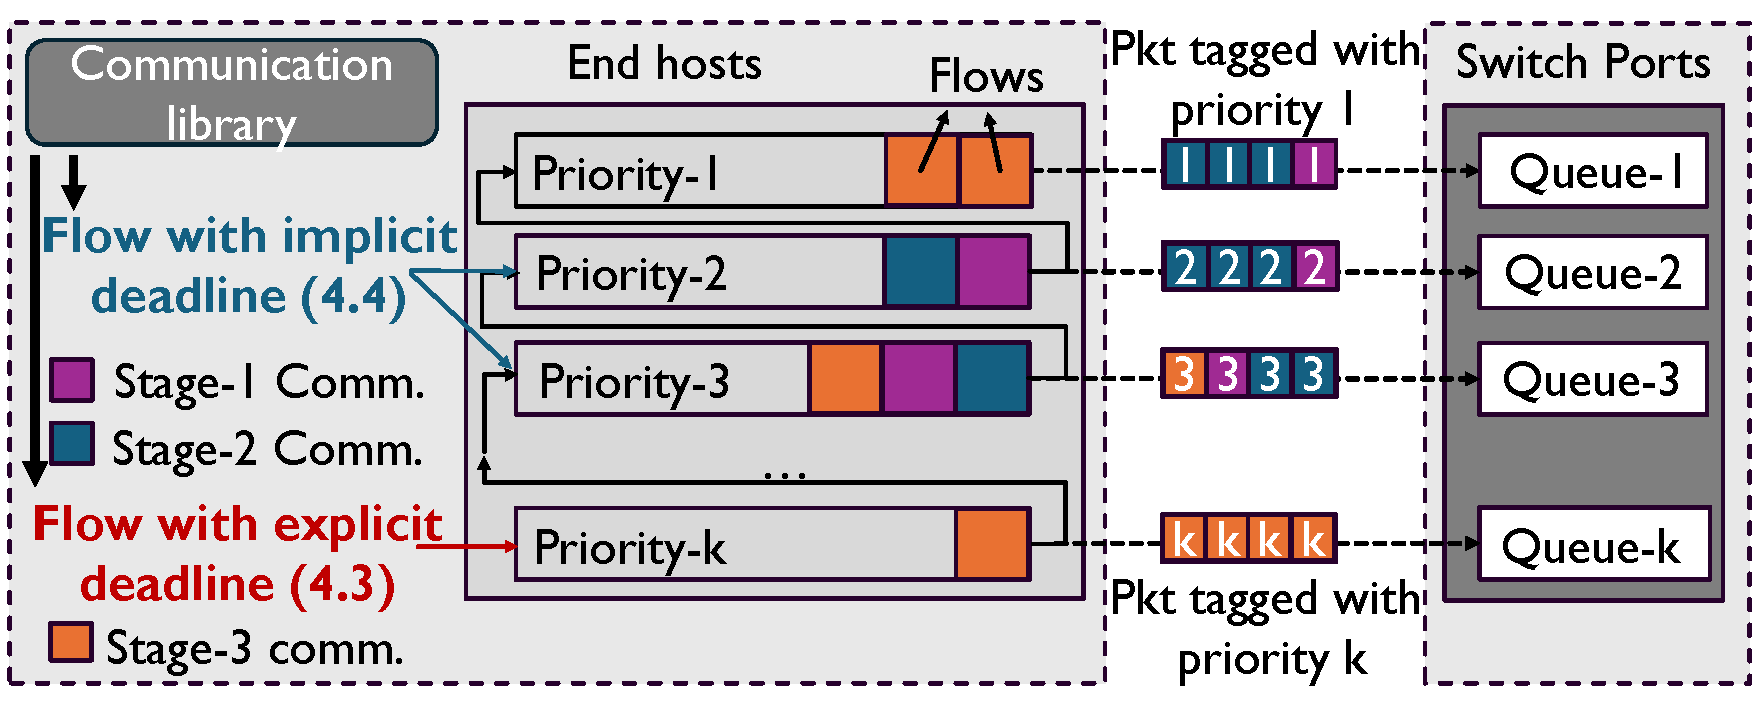
\includegraphics[width=\columnwidth]{figures/design/DesignOverview.pdf}
    \caption{\textbf{设计总览。}}
    \label{fig:design:designoverview}
\end{figure}


\subsection{总览} 图~\ref{fig:design:designoverview} 展示了 \sys{} 的核心抽象：\emph{反向多级队列}（Reverse Multi-Level Queue, RMLQ）。为了实现 \DAP{} 原则，RMLQ 反转了经典 MLFQ 的思路（后者会随着时间推移降低流优先级）；相反，它会先将流放入低优先级队列以体现“延后”，只有当松弛度收紧、必须立刻执行时，才将其提升。

从高层看，\sys{} 通过统一的 RMLQ 底座来调度所有多阶段通信，但针对不同阶段采用不同规则（初始优先级与提升速度）。对于带显式截止时间的末阶段流，\sys 采用最小链路利用率（MLU），只有当剩余带宽刚好不足以满足其截止时间时才提升该流，从而避免过早过度优先。对于带隐式截止时间的早期阶段流，\sys 通过相对层索引（Relative Layer Index, RLI）来推测相对紧迫性。流从较低层级开始，当其可能阻塞计算时再逐步上升。最后，为了解决潜在的跨阶段争用，\sys{} 将最高优先级保留给带显式截止时间的流，以避免违约；其余优先级层则主要用于带隐式截止时间的流，从而机会性地利用可用带宽。

本节剩余部分组织如下：第~\ref{design:explicit} 节介绍带显式截止时间流的调度；第~\ref{design:implicit} 节介绍隐式截止时间情形；最后，第~\ref{sec:design:PET} 节将这些组件整合起来，给出完整的 RMLQ 仲裁逻辑。

\subsection{显式截止时间下的调度}\label{design:explicit}

为应对挑战 C-1，我们需要让末阶段通信任务得到审慎延后——既不过度优先，也不会被饿死——同时严格保证请求截止时间。难点在于，如何将由截止时间导出的连续紧迫度映射到 $K$ 个离散优先级队列上。因此，调度器需要一种机制，用粗粒度优先级近似连续的截止紧迫度，这要求我们回答三个问题：如何量化紧迫度、何时触发提升、以及调度决策应在何种粒度上实施（例如按包还是按层）。

具体地，考虑一个具有 $L$ 层的模型，为一个请求 batch 提供服务。在每一层 $\ell$，P2D 阶段都会产生一组流。同一请求 $r$ 内的流继承其 TTFT 截止时间 $D_r$，而不同请求的流独立调度。我们假设系统有 $K$ 个优先级队列 $P_i(1\leq i \leq K)$，其中 $P_1$ 优先级最高。记将优先级从 $P_j$ 提升到 $P_{j-1}$ 的阈值为 $\tau_j$（$2 \le j \le K$）。我们定义 $\tau_K = +\infty$，以确保即便是极为宽松的流也会落入最低优先级队列。

\parab{紧迫度指标。} 我们定义\emph{最小链路利用率}（Minimal Link Utilization, MLU）：$\mathrm{MLU}_i(t)=\frac{\textit{Size}_{rem}(t)}{\textit{Time}_{rem}(t)\cdot B \cdot (1-\rho)}$，其中 $B(1-\rho)$ 表示扣除背景负载 $\rho$ 后的有效带宽。该指标表示：为了满足截止时间，一个流至少需要占据剩余链路容量的多大份额。关键在于，$\mathrm{MLU}_i(t) > 1$ 表示系统进入不可行的过载状态；数值接近 1 则说明已非常紧急，需要几乎独占的服务；较低取值则意味着仍有足够松弛度可供延后。相较之下，仅基于截止时间的指标（如 EDF）并不适合，因为它们会在过载条件下遭遇多米诺效应~\cite{buttazzo1995value}，在受限于离散优先级层级时还会进一步退化~\cite{buttazzo2005rate}。

\parab{提升阈值优化。} 要推导出能最小化截止违约率的全局最优阈值在计算上是不可行的（NP-hard）。因此，我们转而寻求一种稳健、实用的近似方法：最小化把连续紧迫度映射到离散层级时引入的相对量化误差。当紧迫度为 $v \in [U_{min},U_{max}]$ 的流被映射到离散优先级 $\tau_k$ 时，会产生相对误差 $\epsilon \approx \frac{|v - \tau_k|}{v}$。我们的直觉是最小化所有阈值上的最坏相对误差。由于 $\prod_{k=1}^{K} r_k = \frac{u_2}{u_1} \cdot \frac{u_3}{u_2} \cdot \dots \cdot \frac{u_K}{u_{K-1}} = \frac{u_K}{u_1} = \frac{U_{\max}}{U_{\min}}$，数学上可知，只有当所有比例都相等（$r_k \equiv r$）时，该最坏误差才最小。这要求阈值按几何级数生成（其中 $r =(U_{\max}/U_{\min})^{\frac{1}{K-1}}$）。由于实践中精确的 $U_{\max}$ 和 $U_{\min}$ 往往未知或动态变化，我们通过经验参数近似这一几何间隔：设置提升阈值为 $Q_i = E^{-i}\cdot U$（$1\le i\le K-1$），其中参数 $E$ 与 $U$ 通过经验选取（例如 $E=4, U=0.5$），以获得稳健表现。

\parab{提升行为。}
过细粒度的提升决策会在网络调度中带来现实问题。特别是，如果提升在很细粒度上发生（如按包），同一条消息可能被切分到多个优先级队列中。这会导致分组乱序，即后发包超过先发包，从而触发昂贵的传输层恢复，并降低有效吞吐。为避免这一问题，我们将提升限制在\emph{层边界}上，从而在消息层面保证优先级原子性。关键在于，这种更粗粒度并不会削弱调度表达能力，因为现代 LLM 通常具有很深的网络层数（$L>K$，例如 $L=64$，$K=8/16$），足以提供丰富的优先级调整空间。此外，我们强制采用单调提升策略（即只允许提升）。这可以避免优先级振荡，并进一步强化 \DAP{} 原则：在紧迫性尚未真正达到阈值之前，流会被保守地维持在较低层级。

\subsection{隐式截止时间下的调度} \label{design:implicit}

为应对隐式截止时间情形下缺乏精确松弛度的问题（挑战 C-2），\sys 利用结构性确定性来推断请求内部的相对紧迫度，并通过稳健仲裁机制来解决请求之间残余的争用。

\subsubsection{利用结构确定性的请求内调度}\label{design:intrareq}

尽管由于动态调度偏移的存在，精确松弛度难以获得，但单个请求内部的\emph{相对}松弛度却是确定的：阻塞当前执行的流，必然比只为未来进展做准备的前瞻性传输更紧急。

我们用\emph{相对层索引}（RLI）来量化这一点，其定义为 $\text{RLI} = L_{\text{target}} - L_{\text{curr}}$，其中 $L_{\text{curr}}$ 是当前正在执行的层号，$L_{\text{target}}$ 是该数据被消费的目标层号。较小的 RLI 表示更短的安全延后窗口。\sys{} 通过严格优先调度 RLI 最小的流来解决争用。下面给出两种代表性争用情形。

\parab{情形 I：集合通信与 KV 复用的竞争。} 当 $\text{collective}^{i}$ 与 $\text{reuse}^{j}$（$j > i$）竞争时，集合通信对应当前层（$L_{\text{target}} = i$），因此 $\text{RLI}(\text{coll}) = 0$。相比之下，KV 复用对应第 $j$ 层，故 $\text{RLI}(\text{reuse}) > 0$。因此，我们强制执行 $\text{collective}^{i} \succ \text{reuse}^{j}$，以避免执行停顿。

\parab{情形 II：KV 复用之间的竞争。} 在多层 lookahead 下，$\text{reuse}^{j}$ 与 $\text{reuse}^{k}$（$L_{\text{curr}} < j < k$）常常相互竞争。比较其紧迫性时，第 $j$ 层显然对应更近的截止约束，因此有 $\text{RLI}(j) < \text{RLI}(k)$。优先调度 RLI 更小者能够有效推迟最早执行停顿的发生。因此，我们强制执行 $\text{reuse}^{j} \succ \text{reuse}^{k}$。

总之，\sys{} 通过“严格优先最小 RLI”的统一规则来做出上述决策。定理 1 则形式化说明了这一结构性排序的最优性。

\parab{定理 1。} \emph{在不存在抢占开销的理想计算模型下，严格优先调度 RLI 最小的流，可以最小化 prefill 的总工期。}

\emph{证明思路。} 直观地说，在阻塞区间内优先服务较大 RLI 的流，会浪费本可与后续计算重叠的机会。我们通过交换论证证明这一点：若把任意较大 RLI 的流从阻塞区间中移出，并延后到之后的重叠区间执行，则在不破坏未来依赖关系的前提下，当前阻塞时长会严格缩短。完整证明见附录。

\subsubsection{稳健的请求间调度}\label{design:interreq}

当通过 RLI（第~\ref{design:intrareq} 节）解决了请求内争用后，剩余挑战是：当来自不同请求的竞争流具有相近 RLI，并且同时威胁当前执行时，如何在\emph{请求之间}打破平局。调度器需要在松弛度不精确的前提下，优先保护那些 SLO 违约风险更高的请求。然而，同步 batch 执行会放大调度失误的影响，使错误传播到同一 batch 的所有同伴请求。我们的直觉不是恢复精确松弛度，而是让调度决策对估计误差\emph{更稳健}，从而优先保护那些一旦延迟就会最严重损害 SLO 达成率的请求或 batch。

\parab{松弛度不精确下的调度陷阱。}
我们识别出两类由于误判松弛度而产生的代表性失败案例：
\begin{itemize}[leftmargin=*]
    \item \textbf{Piggyback 效应。} 当一个 batch 内部同时包含极紧和较松的请求时，少数极端紧急请求会主导推断出的 batch 级紧迫性。结果是，同一 batch 中本来宽松的请求也被一并抬高优先级，从而抢占了全局上更紧急的其他 batch。
    \item \textbf{Black Hole 效应。} 距离截止时间近并不意味着它是可完成的。在过载条件下，一个 batch 看起来可能非常紧急，但其负载量已超过可用带宽。优先调度这类 batch 只会把资源浪费在注定失败的任务上，并阻塞其他本可完成的 batch。
\end{itemize}

我们定义\emph{稳健有效截止时间}（Robust Effective Deadline, RED）来量化紧迫性，并对抗 Piggyback 效应。具体而言，我们在 batch 内部按最大截止时间间隔将其划分为“紧请求子 batch”和“松请求子 batch”。记 $D^T_{\text{min}}$ 与 $D^{Lo}_{\text{min}}$ 分别为这两个子 batch 的最小截止时间，则定义 $RED = f \cdot D^T_{\text{min}} + (1-f) \cdot D^{Lo}_{\text{min}}$，其中 $f$ 表示紧请求所占比例。当紧请求比例很小（$f$ 较小）时，$RED$ 会自然偏向较松的截止时间（$D^{Lo}_{\min}$），从而防止少量离群点劫持整个 batch 的优先级。

除基于 RED 的排序之外，我们还采用过载控制来缓解 Black Hole 效应。其直觉在于：避免让注定失败或负担过重的请求阻塞可行请求。我们通过累计估计的计算与通信时延来执行最坏情形可行性检查，并迭代剪除那些对累计时延贡献最大的请求，以恢复剩余 batch 的可行性。

完整算法在附录中给出。它在 batch 到达和离开事件触发时运行，并输出两项结果：(1) 由 RED 决定的有序序列 $\sigma$；(2) 被识别为不可行请求的剪枝集合 $\mathcal{H}$。我们刻意避免在每一层都做细粒度更新，以防调度器对瞬时负载估计抖动产生过度反应。

\subsection{整体整合}\label{sec:design:PET}

\sys 通过统一的 RMLQ 底座调度所有流量。我们根据阶段特征对流进行分类，并针对初始优先级分配与后续提升规则分别做出设计。

\begin{itemize}[leftmargin=*]
    \item 对于带显式截止时间的末阶段流，我们计算第~\ref{design:explicit} 节定义的 MLU 来确定初始优先级。对于提升操作，\sys{} 会在请求计算过程中于层边界更新优先级，而在计算结束后则改为固定时间间隔的周期性更新。
    \item 对于带隐式截止时间的早期阶段流，优先级分配依赖第~\ref{design:intrareq} 节定义的 RLI。阶段 1 流会根据 RLI 进行初始化，并随着计算推进在层边界逐步提升；阶段 2 流则直接进入高优先级队列。
\end{itemize}

\parab{仲裁。} \sys 将最高优先级严格保留给最紧急的末阶段流。在其余优先级层中，\sys 采用分层策略：优先让早期阶段流先于末阶段流，以机会性利用可用带宽；而当多个早期阶段流拥有相同 RLI 时，则按照请求间调度（第~\ref{design:interreq} 节）确定的顺序进行裁决。
